\section{Challenges}
There are several challenges to be taken into consideration while designing a benchmark for SDPSs. In this section we analyse the challenges and provide solutions.

\textbf{ \textit{Simple is beautiful}}. The first challenge is to design a simple system, because simple is beautiful. As the number of systems included inside benchmark increases, the complexity escalades at the same time. One of downsides of the complex system is, difficult to determine the bottleneck. For example, to test the stream data processing engine, the data generator component is essential, to simulate the real life scenarios. Figure \ref{fig_queue_link} shows possible three cases to link data generator and SUT. The simplest design would be connecting the SDPS directly to data generators as shown in Figure \ref{fig_no_queue}. Although this is perfectly acceptable case, it confronts with real life use cases. That is,  in real life, the stream data processing engines, do not connect to pull based data sources unless there is a specific system design. Usually, SDPSs pull data from the distributed message queues which reside between data generators and SUT. One bottleneck on this option is throughput which is bounded by the maximum throughput of message queueing system. We selected the third option which stands between the first two. As can be seen from Figure \ref{fig_partial_queue}, we embedded the queues as a separate module in data generators. In this way, the throughput is bounded only by network bandwidth, the system works more efficient as there are no se/deserialisation overheads and finally it has a simple design. Moreover, while measuring the performance of SUT, using extra systems for checkpointing the current state of measurements or for saving the intermediate evaluation results can affect the SUT's performance.


\textbf{ \textit{Keep driver and test unit as separate as possible}}. The second challenge is to isolate the benchmark driver and SUT as much as possible. For example, in benchmarking SDPSs, it is common to measure the throughput inside the SUT. Because both computations can affect each other the results can be  biased  which we discuss below. We solved this problem by categorising the test unit and pointing measurements accordingly. The first evaluation is throughput. Throughput is associated with the system. So, we kept the throughput assessment outside the SUT, inside data generator module. The second evaluation is latency. The latency is linked with an operator inside system. So, we kept all latency measurements outside the particular operator.

\textbf{ \textit{ Avoid misleading tests}}.
The third challenge is abstain from biased test results and keep the evaluation semantics clear.  One example for this is, throughput measurement. In the previous SDPS benchmarks, the throughput of a SUT is measured by either taking quantiles over test time, or showing max, min and average assessments. From user's perspective on the other hand, the system's throughput is the one with upper bound that it can sustain the data processing. When conducting the experiments with stream data processing engines, back pressure is another factor affecting the throughput, that should be taken into consideration.  Another example for this challenge is latency measurement. In the previous SDPS benchmarks, the latency of an operator is measured by taking difference of tuple's ingestion timestamp to system and output timestamp from system. However, from user's perspective, the start timestamp of a tuple is once it is created and latency of particular tuple should be calculated by taking into consideration its event timestamp. We solve the first issue by measuring the SUT's max throughput that it can sustain under back pressure with a given amount of input. We developed the mechanism for handing the back pressure.  For the second issue, we measure the latency of a tuple by differentiating the time when output is done and its event timestamp.


\textbf{ \textit{ Latency of stateful operator?}} The fourth challenge is measuring the latency of stateful operator. Up to this point, the related works in literature either concentrated on stateless operators or evaluated the latency of stateful operators by checkpointing to external systems like lightweight distributed databases. As we discussed above, this approach can be a bottleneck in some cases. In this paper, we provide a solution for this problem without any external system. 


\begin{figure*}
    \centering
    \begin{subfigure}[b]{0.32\textwidth}
        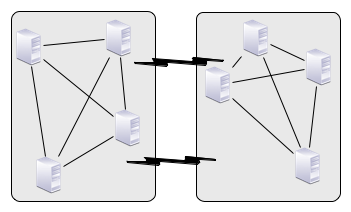
\includegraphics[width=\textwidth]{eps/no_queue}
        \caption{Without message queue}
        \label{fig_no_queue}
    \end{subfigure}
    ~ %add desired spacing between images, e. g. ~, \quad, \qquad, \hfill etc. 
      %(or a blank line to force the subfigure onto a new line)
    \begin{subfigure}[b]{0.32\textwidth}
        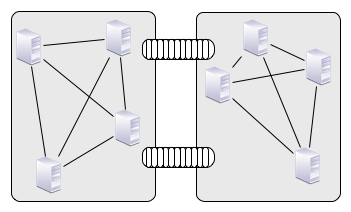
\includegraphics[width=\textwidth]{eps/yes_queue}
        \caption{With message queue}
        \label{fig_yes_queue}
    \end{subfigure}
    ~ %add desired spacing between images, e. g. ~, \quad, \qquad, \hfill etc. 
    %(or a blank line to force the subfigure onto a new line)
    \begin{subfigure}[b]{0.32\textwidth}
        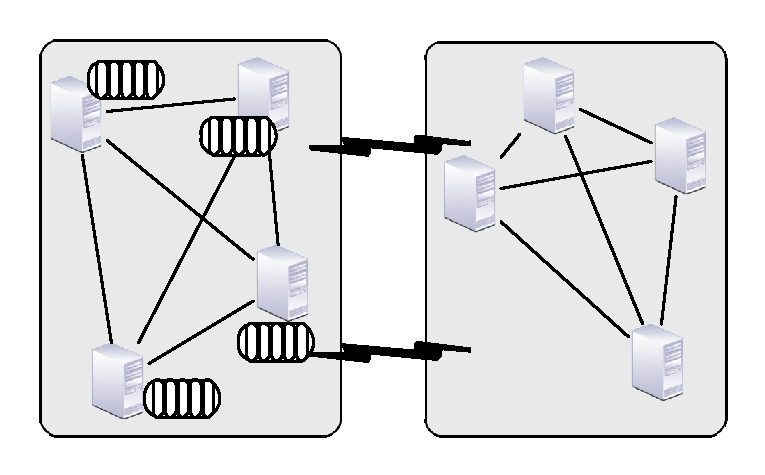
\includegraphics[width=\textwidth]{eps/node_queue}
        \caption{Partial message queue}
        \label{fig_partial_queue}
    \end{subfigure}
    \label{fig_queue_link}
        \caption{Different system designs to link data generator and SUT.}
\end{figure*}
